\section{A ``hand-wavy'' first approach}

What we refer to as Artificial Intelligence is a broad 
collection of methods and techniques used to solve a wide array 
of problems that we collectively associate with ``human 
intelligence'', such as identifying and classifying images, 
processing natural language, and learning from data.  Roughly 
speaking, the discipline can be divided in the following 
sub-fields of research:

\begin{itemize}
	\item Neural Networks.
	\item Vision.
	\item Natural Language Processing.
	\item Speech processing.
	\item Machine Learning.
\end{itemize}

This thesis is concerned specifically with Machine Learning.  
Particularly with a subset of the field known as Reinforcement 
Learning. Some authors such as \cite{SuttonBarto} divide the 
field of Machine Learning (ML) in three parts: supervised 
learning, unsupervised learning, and reinforcement learning.  
Both supervised and unsupervised learning rely heavily in 
statistics-based techniques such as regression models and 
statistical inference. The techniques used in reinforcement 
learning (RL), rely on different models of what learning is, and 
tries to go beyond finding association rules for a simple, 
well-defined problem.

In contrast to supervised learning where a learning agent is 
given data labeled by a knowledgeable source and must ``learn'' 
to classify based on those initial labels, in unsupervised 
learning as well as reinforcement learning, there is no ``train 
data'', the agent must act and optimize it's strategy based only 
upon the reward or penalty resulting from making a certain 
decision.  The key words here being \textit{optimize}, 
\textit{strategy} and \textit{decision}.

For a concrete example picture an android at a casino playing at 
a slot machine, only this machine has $k$ levers instead of just 
one.  This robot is instructed to win as much money as possible 
across some number of games. How could this be achieved? Surely 
each lever makes the machine operate differently and thus is 
more or less likely to get a jackpot. If this were a person, the 
approach would probably be to, across many games, try each lever 
and see how much money comes out. Hopefully, after the first few 
games this human player has a clear idea of which are the best 
levers to pull. This too might be a good strategy for the robot 
to employ, so lets explore that idea further.

If you think about it, the slot machine analogy is not so 
different from the standard mental model we have of say an 
infant learning to crawl.  With poor vision and only it's 
caretaker's voice as guide, it must learn to find its way to 
safety by trial and error. It cannot be given millions of 
examples of ``valid paths'' for extrapolation, as is the case 
with supervised learning. This agent learns by interacting with 
the environment itself.

In a certain sense RL leverages our intuitions about the nature 
of learning. All the main elements are there: cause and effect, 
goals, and consequences to decisions made, but as we will see, 
it also encodes more subtle concepts. For instance, delayed 
gratification and planning ahead. It also has the novelty of 
being goal-oriented rather than task-oriented as most Machine 
Learning techniques often are. For example, a self-driving car 
``trained'' via supervised learning might train on millions of 
examples on what constitutes a valid steering wheel move, while 
one learning by being evaluated is learning how to drive as an 
activity consisting of hundreds of little tasks, all to be 
mastered.

\section{Formalizing ideas}
Now, mathematically speaking, what does it \textit{mean} for a 
machine to ``learn''?

We might not get as far as what learning as a whole means for 
humans or machines, but we can certainly discuss what mechanisms 
allow for things such as self-driving cars and computers beating 
world champions of Chess and Go. For that, we need to identify 
the key concepts in the picture I painted and express them in 
the language of mathematics.

For now, we can gloss over the details of how might a machine 
make decisions, perceive goals, take actions or perceive 
rewards. Let's focus on one key component: the ``learning''. 
When we talk about a machine learning something we are thinking 
about some agent that is able to keep track of the decisions it 
made before and whether or not they resulted in positive results 
so it can later on apply that knowledge to become an 
increasingly better problem solver. If this agent is scored each 
time it carries on some task, we would like for it's score to 
increase each successive time it tries to complete the task. The 
idea of a continually improving score is the foundation of 
mathematical optimization.

\subsection{Optimization Theory}
As the name suggests, mathematical optimization is concerned 
with finding the ``optimal'' solution to problems where an 
unambiguous score might be given to different solutions.  
Whatever ``optimal'' means. Even if there is no best solution to 
a given problem, the techniques used in mathematical 
optimization often allow for a continual improvement through 
iteration.

Going back to our slot machine example, each time the robot 
selects one of the $k$ levers the machine gives out a prize. The 
prizes vary greatly in size, and there is no way to know which 
ones give the biggest prizes in advance. Since the robot wants 
to maximize money earned, if one lever is consistently resulting 
in bigger prizes it is likely to keep pulling it. The robot was 
rewarded earlier for choosing that lever by getting a big prize.  
Similarly if a lever pull resulted in no prize at all, the robot 
lost money by playing and probably won't choose that lever 
again. In each iteration the player robot would like to increase 
more and more the prize, and thus is encouraged to keep track of 
which levers give good prizes, improving the average prize in 
each successive game.

We are now ready to peel away another layer of abstraction.  We 
now have an intuition of what it means for a machine to learn, 
or in other words continually improve. But in the model we 
discussed earlier, the player is making choices along the way. A 
predefined path is not programmed or even known. If it were 
known this wouldn't be a problem at all, the robot could choose 
the known-good levers every single time. Since that is not the 
case the robot must choose and balance between exploring and 
exploiting what knowledge was gained so far. What does it mean 
for this player robot to ``make choices''?

\subsection{Stochasticity}
Another key aspect we take for granted when we talk about 
machines learning is implicit in the word learning. If there 
were a predefined path for the robot to take we would hardly 
call that learning, it's merely reproducing instructions.  What 
this means for us, is that we must allow for a framework in 
which our robots actions are not completely determined 
beforehand. In fancier words, the succession of events that 
determine the robots actions and responses to stimuli are not 
predetermined or \textit{deterministic}.

This idea is formalized through something called a 
\textit{stochastic process}. The word stochastic is just 
mathematician speak for ``not entirely determined beforehand'' 
or ``aptly described as a random phenomena''.  In particular, we 
can think of the robot as being in some state among many many 
possible. The robot can change states as time goes by but the 
transitions are not always the same and they don't necessarily 
always carry the same reward or punishment.

For instance, the robot on the slot machine might have gotten a 
very big prize the first time it chose a certain lever but got 
almost nothing the next game. The feedback it got by choosing an 
action changes as time goes by, the slot machine behaves 
randomly. This robot had a certain information after pulling the 
lever for the first time: this is a good lever to pull. On the 
next game this robot already knows which lever might be a good 
bet, so among the $k$ possible options it might choose to pull 
the same lever as last time. Next time the reward is much 
smaller. This robot transitioned states in a sense. It was in a 
state were the best option was somewhat clear, to a state in 
which that one lever is no longer the most desirable option. It 
went from being certain to being forced to explore. We might 
think of this process a navigating the branches of a tree, 
making a decision every time a branch forks of into smaller 
branches.

[AQUI DIAGRAMA DE ARBOL]

\section{A slightly more nuanced example}
One of the major achievements and claims to fame for 
reinforcement learning in the past decades has been its use in 
some of the most famous matches in several classic board games.  Chess was 
``mastered'' when Kasparov was beat by Deep Blue in 1997 
\cite{silverchess}, but other board games with enormous state 
spaces such as Go, the game that originated in China, proved to 
be too complex for the techniques used by Deep Blue. Go was much 
later attacked by another robot player named AlphaGo developed 
by DeepMind researchers \cite{silver2017mastering}.  AlphaGo 
defeated Lee Sedol, the reigning human champion in 2016.  
AlphaGo was one of the most notorious applications of RL and 
made the field even more popular. Since RL has proved to be very 
good for these kinds of tasks in the past, let's explore an 
example with a simpler board game.

\subsection{Duopoly, oligopoly, \ldots}
Lets consider a simplified version of a popular game whose name 
I don't know if I can use as it might be copyrighted. This game 
consists of a circuit with predefined squares in which a player is 
at any given moment or turn. The player moves by spinning an 
arrow that can land on any number from 1 to 4, and moves forward 
the number of squares that the spinner landed on. A The robot might 
acquire that square for itself and if it lands on it again, gains 
some amount of money. The robot also receives money every time 
it completes the circuit. In this simplified version the robot 
is playing alone, but every turn some square the robot doesn't own 
might become unavailable for purchase, and the robot must pay if 
it lands on it from then on. If it lands on jail the robot also 
loses money, a bigger amount. As you might have guessed, the 
point of the game is to make the most amount of money. The game 
ends when the robot goes bankrupt or the amount of squares that 
the robot can buy runs out. What purchase strategy must the 
robot follow to win?

\begin{figure}[H]
	\centering
	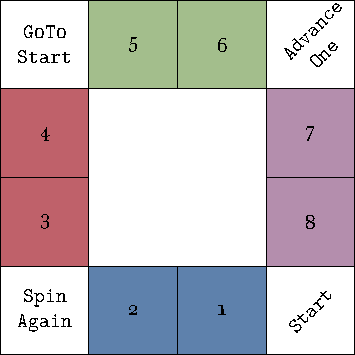
\includegraphics[width=.75\textwidth]{img/board.pdf}
	\caption{Board for the game described earlier}
	\label{fig:miniopoly-board}
\end{figure}

First off, unlike the slot machine-playing robot, this robot 
player cannot entirely choose which square to move to, it can 
only decide if it wants to purchase it or not once it landed on 
it.  For instance, if we look at Fig. \ref{fig:miniopoly-board} 
we see that even if the robot wanted to go to square number 8 
and buy it there is no possible way to do that. The biggest 
number it can spin is 4, and even if it got to roll again the 
furthest it could go is square 5. Let's revise the board and 
simplify by removing the squares that are not accesible on the 
first spin, and lets draw some arrows to make the transitions 
clearer.

\begin{figure}[h]
	\centering
	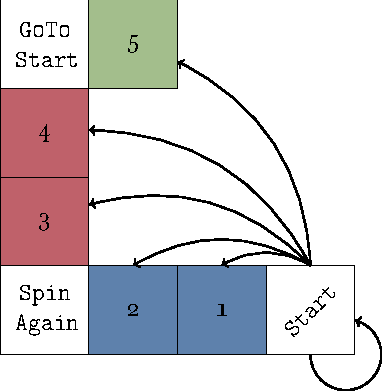
\includegraphics[width=.75\textwidth]{img/diagram-start.pdf}
	\caption{Squares accessible on the first spin}
	\label{fig:miniopoly-diagram-start}
\end{figure}

On fig. \ref{fig:miniopoly-diagram-start} we can see all the 
possible squares the robot might land on and then buy starting 
from the first spin. Notice how for instance there is an arrow 
that points from ``Start'' to itself. This transition might 
happen. In fact we know what it takes for it to happen: land on 
``Roll Again'', and then land on ``GoTo Start''. In other words, 
this transition happens if the robot spins a 3 two consecutive 
times. Notice how in this diagram we only care about the 
starting and ending points, not the transit points, so that's 
why there are no arrows pointing to the squares what move the 
player elsewhere. 

That particular move results in the robot going back to the 
start and getting paid for completing the circuit, without 
running the risk of landing on a square someone owns and getting 
charged. That sounds like a very desirable play (for us looking 
at the big picture, the robot can't see that far ahead yet).  
Since we would like this to happen, we might ask how likely is 
for that to happen.

\begin{figure}[h]
	\centering
	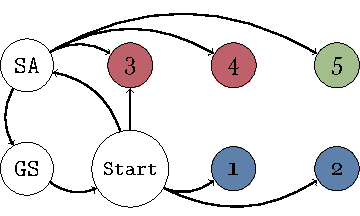
\includegraphics[width=\textwidth]{img/transicion.pdf}
	\caption{Transition diagram}
	\label{fig:miniopoly-transicion}
\end{figure}

Lets try to analyze how likely the robot is to end up in this 
particularly rewarding situation. For that it's often helpful to 
think of the possible steps that lead to it. On figure 
\ref{fig:miniopoly-transicion} we can see a more abstract 
diagram of the possible movements the robot might make, and this 
time we are taking into account intermediate squares. Each arrow 
represents where the robot might land after spinning, not 
necessarily where it is when the turn ends. Now, using some very 
basic probability theory we can calculate how likely it is for 
the robot to ``take that route'' so to speak. Once we do, we can 
calculate how likely a ``trajectory'' or sequence of arrows is.

\begin{figure}[h]
	\centering
	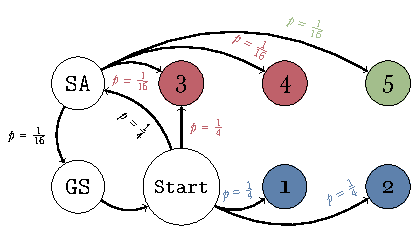
\includegraphics[width=\textwidth]{img/transicion-markov.pdf}
	\caption{Transition diagram with transition probabilities}
	\label{fig:miniopoly-transicion-markov}
\end{figure}

At the moment it is not important why some arrows have certain 
probabilities, and some might not be terribly obvious even for 
someone acquainted with some basic probability. In diagram 
\ref{fig:miniopoly-transicion-markov} to find the probability of 
getting to a certain square (say 6 for example) we look only at 
the last arrow, as it takes into account the probability of the 
last step happening.

The robot we are trying to teach moves as the diagram above 
suggests. For each square there is a different diagram. The 
robot is not aware of this, all it knows is that it spins, and 
then is transported elsewhere and must decide whether to buy or 
not (if the square is available). All it knows is where it has 
been before and if it gained or lost money last turn. Crucially, 
landing on a square previously visited does not necessarily mean 
the reward will be the same as last time. Also, the reward for 
buying a square may come much later on or not at all. This 
student must somehow keep track of what the expected reward for 
landing somewhere might be, recording it somewhere and tallying 
up as it goes. For instance after a few turns it might have 
something fig. \ref{fig:hist-miniopoly} on its head to help make 
decisions.

\begin{figure}
\centering
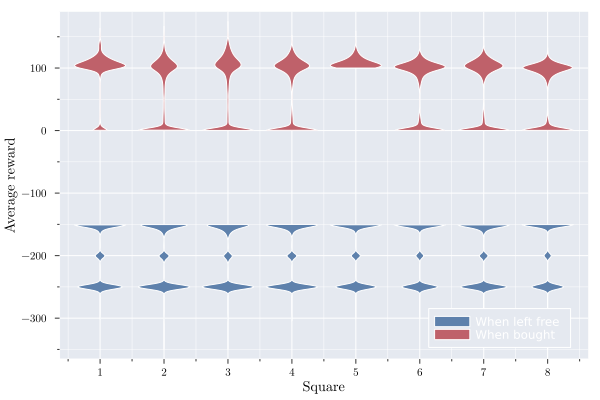
\includegraphics[width=\textwidth]{img/hist-miniopoly.tikz}
\label{fig:hist-miniopoly}
\caption{Histogram of rewards obtained by visiting each square}
\end{figure}

Its stands to reason that as this histogram is updated the 
learning agent will be able to make progressively better 
choices. Simple as this example might be, the essence is similar 
to the powerful programs that beat world champions.

This example covers most of the core ideas of what is referred 
to as the Reinforcement Learning Problem. We will explore the 
ideas presented here in much more detail along this theses and 
crucially, focus on something we left out on this example. How 
can a purchase strategy be improved upon?

\section{Wrapping up}
So far we have developed a mental model of what to do should we 
wish to teach a robot how to drive or beat a world champion of 
Go. The rest of this thesis is dedicated to the careful 
development of the ideas here presented into the language of 
mathematics.  But beyond mere description, this exercise has the 
potential to unlock \textit{insight}. As is often said by 
legendary math communicator Grant Sanderson\footnote{From the 
	YouTube channel 
\href{https://www.youtube.com/channel/UCYO_jab_esuFRV4b17AJtAw}{3blue1brown}}(loose 
quote), the point in formulating things this way is to gain a 
deeper understanding of the phenomenon. So let's dive right in.
